\documentclass[a4paper, 11pt]{scrartcl}
\usepackage{fullpage}
\usepackage{graphicx}
\usepackage{appendix}
\usepackage{booktabs}

% hyperref and nameref so that we can have sane internal refs
% hyperref also helps with pdf index creation
\usepackage[linkcolor={blue},citecolor={blue},urlcolor={red}]{hyperref}
\usepackage{nameref}

% Place all of the figures at the end of the document
\usepackage[figuresonly,nomarkers,nolists]{endfloat}
\renewcommand{\efloatseparator}{}

% Set to false for black/white printing
\hypersetup{colorlinks=true}

\title {Student Robotics 2013\\ Rulebook}
\author{Revision 4}
\date{\today}
\setcounter{tocdepth}{1}

\begin {document}
\maketitle

\noindent The following defines the rules and regulations of the Student Robotics 2013 competition.

\newcounter{rule}[section]
\newcommand{\rcn}{\stepcounter{rule}\arabic{section}.\arabic{rule}}
\renewcommand{\labelenumi}{\rcn}

\section {Game Rules}
\label{game-rules}

\begin{enumerate}
\item The game, called \textbf{Caldera}, will be played in the arena defined in section~\ref{sub:arena}.  The objective of this game is to capture the most zones -- especially tricky, hard-to-reach ones -- and keep your opponents from doing the same.

\item Before a match begins, participating teams must:
\begin {enumerate}
  \item Present their robot in the staging area, adjacent to the arena, at least 2 minutes before the scheduled start time.
        The staging area will be clearly marked on the day.

  \item Attach four robot badges.
        These badges will be provided by Student Robotics officials in the staging area.
        Section~\ref{sub:robot-badges} provides more information about these badges, as well as their dimensions and mounting requirements.

  \item Place their robot in the starting zone that they are assigned.
        The robot must be placed such that it is entirely within this starting zone, with no parts overhanging its boundary.

  \item Vacate the arena 40 seconds before the scheduled start time.
        During the 40 second period prior to the start of the match there must be no interaction with the robot.
\end{enumerate}
  Teams that fail to comply with this rule--such as by arriving late--may forfeit the match, at the discretion of the judge.

\item A match lasts 150 seconds.

\item There will be a maximum of 4 robots in a match.

\item Robots will be started by teams leaning into the arena to press the start button on their robot\footnote{A wireless match-starting solution may be provided by Student Robotics.} when instructed to do so.

\item A match may be terminated prematurely if all teams participating in that match state to the match officials that they are happy for the game to end.

\item There are 25 scoring zones in the arena, arranged in a $5\times5$ grid. The outer 16 are known as the ``base'', the inner 8 are known as the ``volcano'', and the most central zone is known as the ``caldera''. The volcano (and, notably, \emph{not} the caldera) is elevated from the floor by $75 mm \pm 5 mm$.

\item There are 40 tokens in the arena: 10 per team. These tokens are marked for the starting zone with which they are associated. These are initially placed in 5 stacks of 2 high, along the wall to the right of the robot's starting position, as defined in section~\ref{sub:arena}.

\item A scoring zone is deemed ``captured'' by a team if and only if that team has the single\footnote{Were two teams to have the same number of tokens in a scoring zone, the zone would not be considered captured by any team.} most tokens ``in'' the zone at the end of the game.

\item A token is considered to be `in' a zone if either:
\begin{enumerate}
  \item at least three vertices of the token are in contact with the floor area inside the zone. The floor area inside the zone is bounded by the edges of the raised volcano, and the inside edge of the coloured tape marking the zone.
  \item the token is in contact only with other tokens which are `in' the zone. In the case where several such tokens are in mutual contact (and not in contact with anything else), all those tokens are `in' the zone.
\end{enumerate}

\item Captured zones in the base are worth \textbf{2 game points} each. Captured zones on the volcano are worth \textbf{7 game points} each. The caldera, if captured, is worth \textbf{30 game~points}.

\item If, at the end of the game, a robot is ``in'' a zone, the value of that zone and the four zones immediately adjacent in the cardinal directions are tripled. This effect compounds with multiple robots, meaning that it is possible for the value of a zone to be increased 81-fold in one theoretical case.  % When a robot is 'in' a zone is explicitly undefined and will be made by a ruling at the competition

\item At the end of a game, league points will be awarded as follows.
      The team with the \emph{most} game points will be awarded 8 points towards the competition league.
      The team with the second most will be awarded 6.
      The team with the third most will be awarded 4 points, and the team with the fewest game points will be awarded 2 points.
      Teams whose robot was not entered into the round, or who were disqualified from the round, will be awarded no points.

      Tied robots will be awarded the average of the points that their combined positions would be awarded.
      Thus, three robots tied for first place would receive 6 points each (since this is $(8+6+4)/3$).

\item Once the league has completed, a knockout competition will begin.
      The positions of the teams in the league will seed the positions of teams in the knockout matches.
      The top teams from the league advance to the knockout.
      The number of teams progressing to the knockout will be announced before the start of the league matches.
      In the event of tied league positions, the team with the greatest cumulative game points in the league will go through.

      Each match in the knockout competition involves up to 4 teams.
      The teams that come 1\textsuperscript{st} and 2\textsuperscript{nd} in each knockout match will continue to the next round of the knockout.
      In the event of a tie in a knockout match, the team that ranked highest in the league will go through.
      If there is a tie in the final, then a rematch will be played.
      The number of league and knockout matches will be announced on the morning of the competition.

\end{enumerate}

\newpage
\section {Regulations}
\label{sec:Regulations}

\begin{enumerate}

% Overarching safety

\item All robots must be safe.

\begin{enumerate}
  \item It must not be possible to directly or indirectly injure oneself on the robot.
        Exposed sharp edges and fast moving parts, for example, will be tested using a Frankfurter sausage to simulate a finger.
        Teams are encouraged to discuss any safety concerns about their robot on the Student Robotics forums.

  \item The robot's power switch must be on the outside top of the robot and easily accessible at all times -- including throughout the game.
        This is for everyone's safety, especially your robot's.

  \item The lithium-ion polymer batteries provided in the kit must be shielded from mechanical and thermal harm.
        This includes mechanical protection from accidental impact with other robots.
        Teams found to be in violation of this rule will have their batteries confiscated until they have demonstrably rectified the identified issues.

  \item Only the power board may be connected directly to the battery.
\end{enumerate}

%% Meta

\item The Judge's decision is final.
\item Any assistance from Student Robotics volunteers is provided without guarantees.
\item Student Robotics reserves the right to examine your robot software and hardware at any time.

%% Behaviour

\item No remote control systems may be used.
\item This is a non-contact sport, but accidental bumps and scrapes are inevitable.
\item Robots must not intentionally damage anything -- including tokens, zone barriers, the arena or other robots.
      At the discretion of the judge, teams who deliberately engage in collisions or take insufficient precautions against collisions may be penalised, including disqualification from rounds and deduction of league points.
\item All kit deployed by Student Robotics remains the property of Student Robotics.
      All electronic kit \textbf{must} be returned to Student Robotics after the competition.
      \autoref{sec:kit-return} details the parts of the kit that must be returned.
      After the competition, the kit that is not specified in \autoref{sec:kit-return} becomes the property of the team.

%% Physical

\item Robots must pass an inspection by a Student Robotics Inspector before competing in a match.
      This inspector will check that the robot complies with the rules and regulations of this game, and is safe to compete (see \autoref{sec:safety-regs}).
      \textbf{Robots that have not passed inspection will not be permitted to compete}.

\item At the beginning of each match, robots must fit within a cube with $500mm$ internal sides.
      \textit{During the match}, the robot may extend beyond this size.

\item During a match robots may deploy supporting equipment into the arena, as long as that equipment is clearly designed to be of direct benefit to the robot.
      Such equipment must not deliberately impede other robots and reasonable care must be taken to ensure that it does not become merely an obstacle to other robots.

\item All wires connected to the robot's ground (0V line) must be black.
      Black wires \emph{must not} be used for anything else.
      It is \emph{strongly recommended} that all wiring is neat and easily removable, as this will reduce the time required to debug problems on robots
       (teams may be asked to tidy their wiring before a Student Robotics volunteer will approach any issues with their robot).

\item All electronics must be securely fixed to the robot, and should also be easily removable.

\item All robots must have mountings for the removable robot flags
      provided by Student Robotics, as described in section~\ref{sub:robot-flag}. A mounting
      must firmly hold a flag in an upright position. Flags must be mounted on the top of the robot.

\item If teams wish to use batteries other than the lithium-ion polymer batteries provided,
       then they must seek approval from Student Robotics through the Student Robotics forums first.
      Additionally, if teams wish to add systems powered by separate batteries then they must seek approval through the same channel first, with the exception of video cameras.

      In general, teams are encouraged to power everything off the Student Robotics supplied battery through the power board.

\item Robots may not include radio transmitters or receivers.
      In exceptional circumstances, teams may request an exemption from this rule.

\item Robots must not have any devices designed for the sole purpose of producing audible noise, with the exception of the piezoelectric buzzer on the power board.

\item Robots must have a spare USB slot to be used by the competition USB provided by Student Robotics, which is inserted during staging. This slot will be in addition to the slot used for user's robot code, and must be easily accessible. Robots without a competition USB may not enter a match.

\end{enumerate}

\newpage
\section{Specifications}
\label{sec:Specifications}

\newcounter{rulei}[subsection]
\newcommand{\rcnii}{\stepcounter{rulei}\arabic{section}.\arabic{subsection}.\arabic{rulei}}
\renewcommand{\labelenumi}{\rcnii}

\subsection{Markers}
\label{sub:markers}
The arena, tokens, slots, and robots involved in the game are labelled with \textit{libkoki} markers.
Each marker pattern encodes a number.
Each marker number is associated with a particular feature within the arena, and also has an associated size.
The marker numbers and sizes are as follows:

\begin{center}
  \begin{tabular}{lcc}
    \toprule
    \textbf{Item} & \textbf{Marker Numbers} & \textbf{Marker Size (mm)} \\
    \midrule
    Arena boundary & {} 0 -- 27 & 250 \\
    Robots & 28 -- 31 & 100 \\
    Slots & 32 -- 39 & 160 \\
    Token Top & 40 -- 43 & 160 \\
    Token Bottom & 44 -- 47 & 160 \\
    Token Side & 48 -- 51 & 160 \\
    \bottomrule
  \end{tabular}
\end{center}

Two sets of marker codes will be used: one for development purpose, and one for the competition itself.
The competition set is only to be used inside the Student Robotics arena at the Student Robotics competition.
This is so that people carrying markers past the arena do not confuse robots.
The competition codes are 100 above the development codes.
When run in competition mode (specifiable through the robot's GUI), the software provided by Student Robotics will subtract 100 from the detected marker codes, as well as ignore the development codes.

The markers can be printed on a black-and-white printer.
Marker designs can be downloaded from the documentation section of the Student Robotics website.

Unless specified otherwise, all markers described in this document are oriented vertically such that the principle corner of the marker (which is indicated by a dark grey dot in the black marker border) is on the higher edge.

\subsection{Robot Badges}
\label{sec:robot-badges}

\begin{figure}
  \centering
  
\includegraphics[width=\textwidth]{./images/robot-marker.pdf}
  \caption{An example robot badge.
           The blue areas shown are the human-compatible areas.
	   All dimensions are in millimetres.}
  \label{fig:example-badge}
\end{figure}

\begin{enumerate}
\item A ``robot badge'' is a removable identifier that will be attached to a robot throughout a match.
      It features the robot's assigned marker for the match, as well as human-compatible areas to allow spectators to easily associate a robot with its starting location.
      An example of one of these badges is shown in figure~\ref{fig:example-badge}.
      The markings in the human-compatible areas are intentionally not specified.

\item A robot must feature four of the badge mounts shown in figure~\ref{fig:badge-mounting}.
      These mounts must permit a flat $200 \times 100mm$ panel to be attached to them.
      The three areas of each mount must feature the illustrated areas of hook-type Velcro to allow this panel to be fitted.

\item The four badge mounts must be on the exterior of the robot, parallel with the vertical plane, and should be perpendicular to each other about the vertical axis\footnote{Teams can apply for a team-specific rule alteration to the required number of badges.
      Clear justification must be provided by the team with such a request.}
      The orientation of the badge mounts is unimportant, but teams are encouraged to position them horizontally as shown in figure~\ref{fig:example-badge}.

\item The mapping between a given robot and its robot badge is as follows:

\begin{center}
  \begin{tabular}{cc}
    \toprule
    \textbf{Corner} & \textbf{Marker Number} \\
    \midrule
    0 & 28 \\
    1 & 29 \\
    2 & 30 \\
    3 & 31 \\
    \bottomrule
  \end{tabular}
\end{center}

\begin{figure}
  \centering
  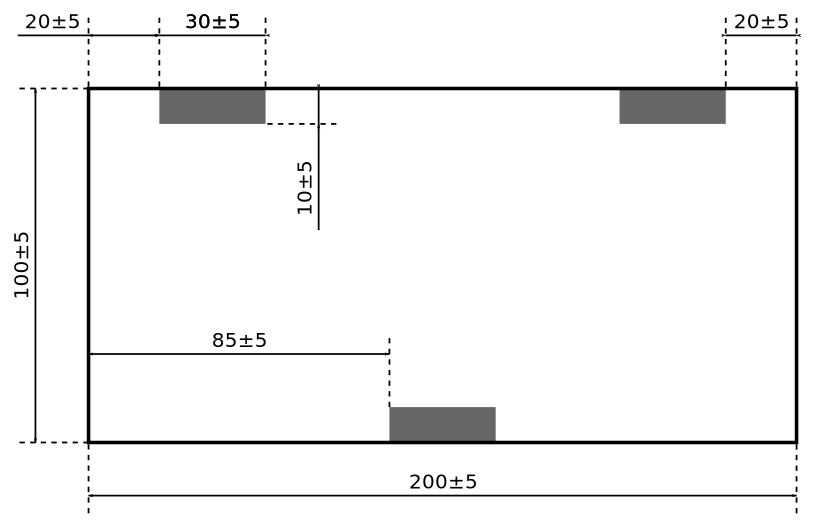
\includegraphics[width=\textwidth]{./images/badge-mounting.pdf}
  \caption{The dimensions of the required robot badge mountings.
           The shaded areas are hook-type Velcro.
           All dimensions are in millimetres.}
  \label{fig:badge-mounting}
\end{figure}

\end{enumerate}

\subsection{Arena}
\label{sub:arena}
\begin{enumerate}
\item The match arena floor, overall, is an $8m \times 8m$ square, as shown in figure~\ref{fig:arena-dim}.
      The tolerance of these two dimensions is $\pm0.25m$.

\begin{figure}
  \centering
  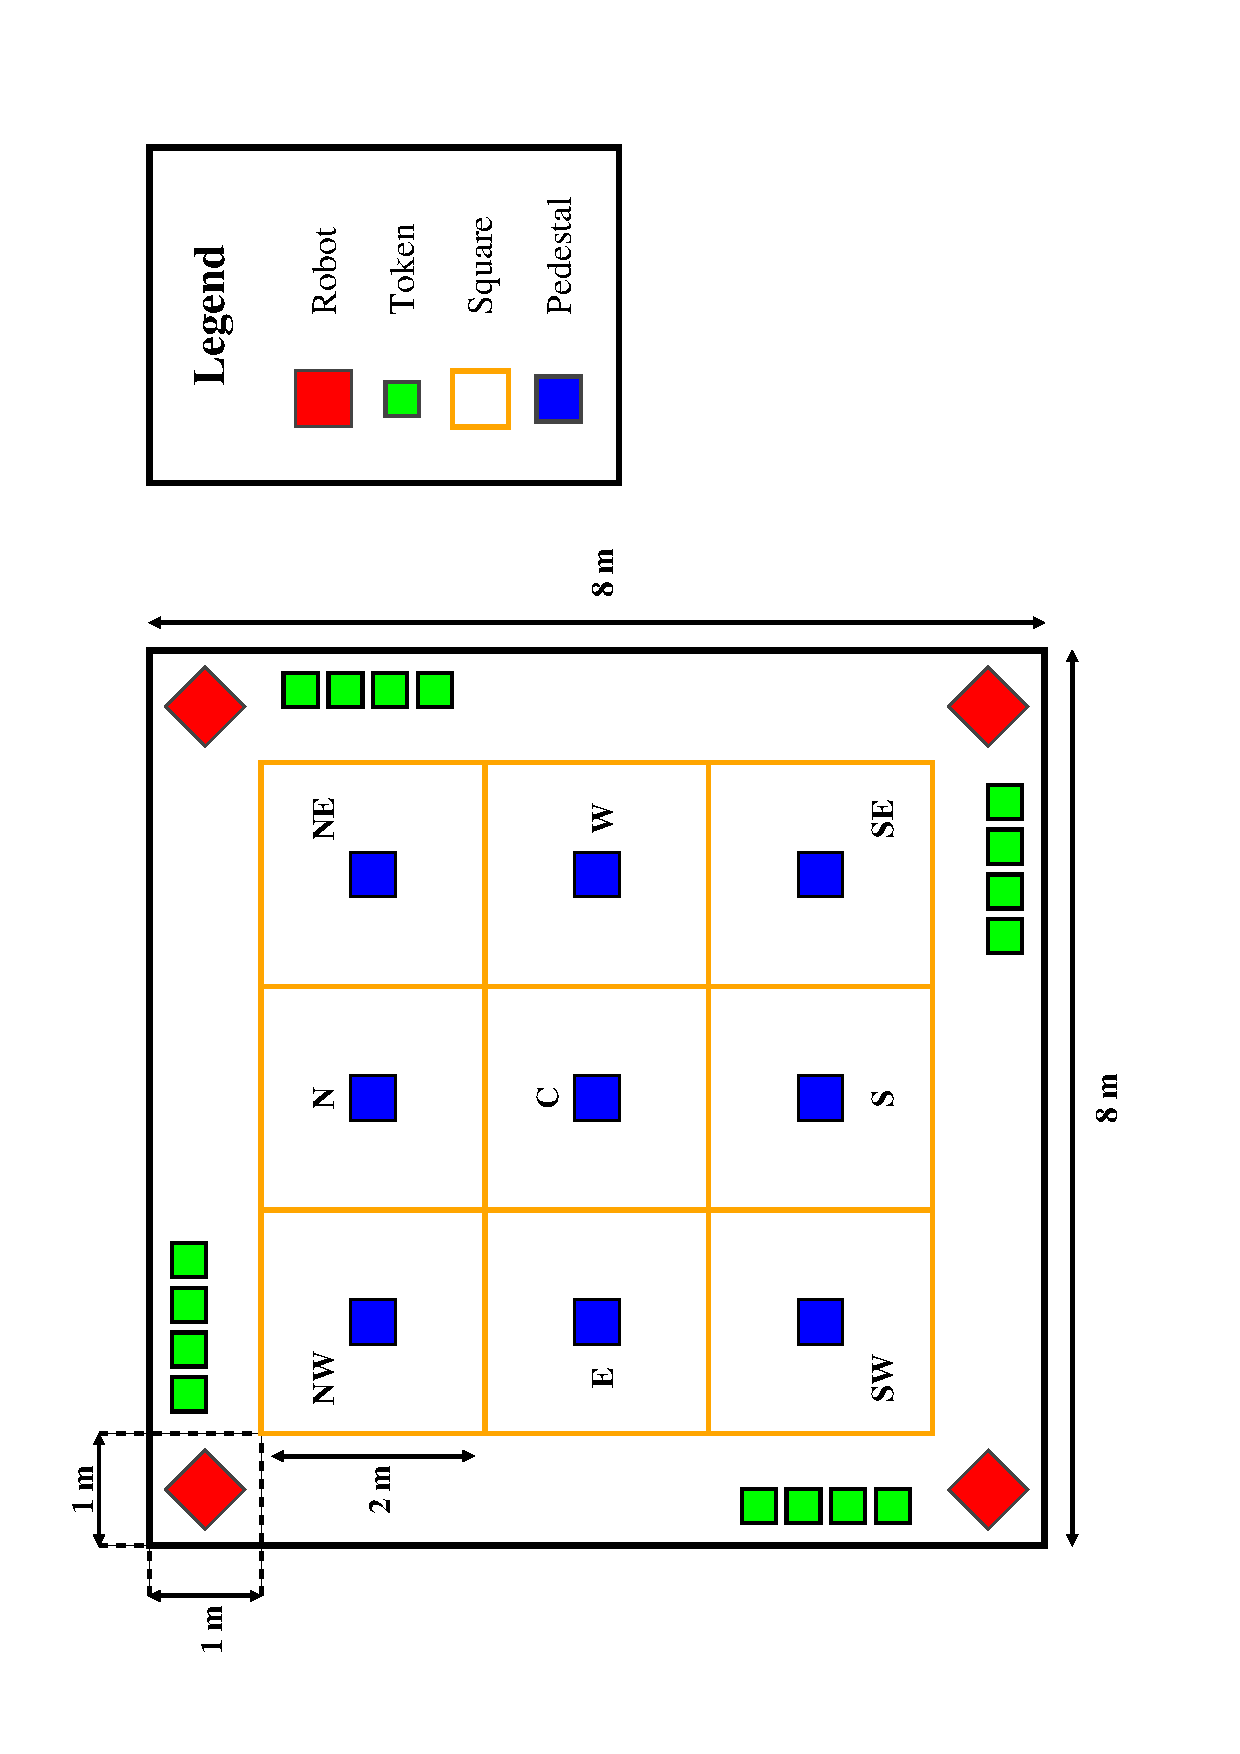
\includegraphics[width=\textwidth]{./images/arena.pdf}
  \caption{\label{fig:arena-dim}A bird's-eye view of the arena. All dimensions are in millimetres.}
\end{figure}

\item The floor of the arena is carpeted with blue carpet tiles.

\item The arena walls are $600\pm30mm$ high, the interior surfaces of which are white plastic-coated hardboard.

\begin{figure}
  \centering
  
\includegraphics[width=\textwidth]{./images/sidewall.pdf}
  \caption{Seven $250mm$ wide markers are spaced evenly along each $8m$ arena wall.
           The markers are placed $50mm$ above the floor.
	   All dimensions are in millimetres.}
  \label{fig:arena-wall}
\end{figure}

\begin{figure}
  \centering
  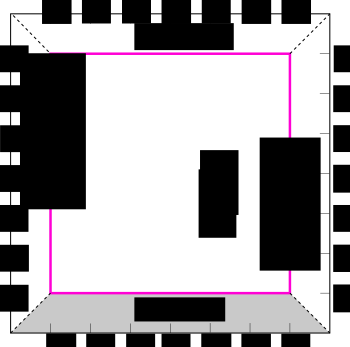
\includegraphics[width=0.5\textwidth]{./images/arena-markers.pdf}
  \caption{Twenty eight arena wall markers are positioned around the perimeter of the arena with the marker codes incrementing in an anti-clockwise fashion.
           The corners are counted in a clockwise fashion, with corner 0 being the corner closest to arena marker 0.}
  \label{fig:arena-zones}
\end{figure}

\item Each wall of the arena features seven $250mm$ libkoki markers.
      Figure~\ref{fig:arena-wall} shows the positioning of these markers, whilst figure~\ref{fig:arena-zones} shows the numbering of these markers.

\item Each robot will be assigned a corner at the start of every match to indicate its starting position.
      Corner starting positions are $1000 \pm 20mm$ square and will be marked by $25mm$ paper-based masking tape.
      The mapping of these corner numbers in the arena is shown in figure~\ref{fig:arena-zones}.

\item Student Robotics reserves the right to have up to three match officials in the arena during games.

\end{enumerate}


\subsection{Zones}
\label{sub:Zones}

\begin{figure}
  \centering
  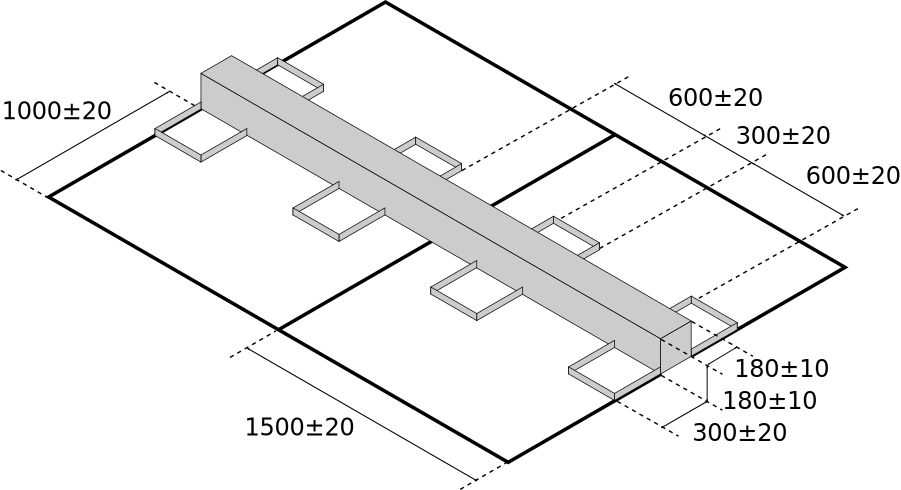
\includegraphics[width=\textwidth]{./images/slots-zones.pdf}
  \caption{The arena contains four zones, each $1500 \pm 20mm$ wide and $1000 \pm 20mm$ deep.
           The rectangle described by the four zones is split in two by a $180 \pm 10mm$ high, $180 \pm 10mm$ deep zone wall.
           Eight $25 \pm 5mm$ high slots---two in each zone---are attached to the zone wall.
           All dimensions are in millimetres.}
  \label{fig:slots-zones}
\end{figure}

\begin{enumerate}
\item There are four zones in the centre of the arena.
      The arrangement of these zones can be seen in figure~\ref{fig:arena-dim}, and is shown in more detail in figure~\ref{fig:slots-zones}.

\item Each zone is $1500mm$ wide and $1000mm$ deep and is  marked with $25mm$ wide paper-based masking tape.

\item A single $180 \pm 10mm$ high, $180 \pm 10mm$ deep wall splits the four zones in two.
      The position of the wall can be seen in figure~\ref{fig:slots-zones}.
\end{enumerate}


\subsection{Slots}
\label{sub:slots}

\begin{enumerate}
\item There are eight slots in the arena.
      Two slots appear in each zone, as shown in figure~\ref{fig:slots-zones}.

\item Each slot is identified by a unique $160mm$ libkoki marker (see section~\ref{sub:markers}).
      Slot markers are affixed to the zone wall, each centered in their corresponding slots, and $20 \pm 5mm$ above the floor.

\item Slots are attached to the zone wall.

\item The boundary of each slot is constructed using square cross-sectioned wood with a side length of $25 \pm 5mm$.

\item Externally, each slot is $300 \pm 20mm$ wide and $300 \pm 20mm$ deep.

\end{enumerate}


\subsection{Tokens}
\label{sub:Tokens}
\begin{enumerate}
\item Tokens are cubic corrugated cardboard boxes with side $200 \pm 15 mm$.
      \emph{Each team's kit contains two of these.}

\item Each robot has eight identical tokens associated with it, two in each corner.

\item A token for a given robot will be labelled with three distinct $160mm$ libkoki markers: one for the top, one for the bottom, and four identical markers for the remaining sides.

\item Token side markers are oriented such that the top left corner of each marker (identified by a small grey dot) is affixed to the top left of a token's side face, with the top and bottom markers affixed accordingly.

\item Tokens will be styled to match the human-compatible area of the robot badges on their associated robot, allowing spectators to follow game play.
      See section~\ref{sec:robot-badges}.

\item The mapping between a given robot and its associated markers is as follows:

\begin{center}
  \begin{tabular}{cccc}
    \toprule
    \textbf{Corner} & \textbf{Top Marker} & \textbf{Bottom Marker} & \textbf{Side Markers} \\
    \midrule
    0 & 40 & 44 & 48 \\
    1 & 41 & 45 & 49 \\
    2 & 42 & 46 & 50 \\
    3 & 43 & 47 & 51 \\
    \bottomrule
  \end{tabular}
\end{center}

\item Tokens will initially be positioned to the left and right of the robot as shown in figure~\ref{fig:token-position}.

\begin{figure}
  \centering
  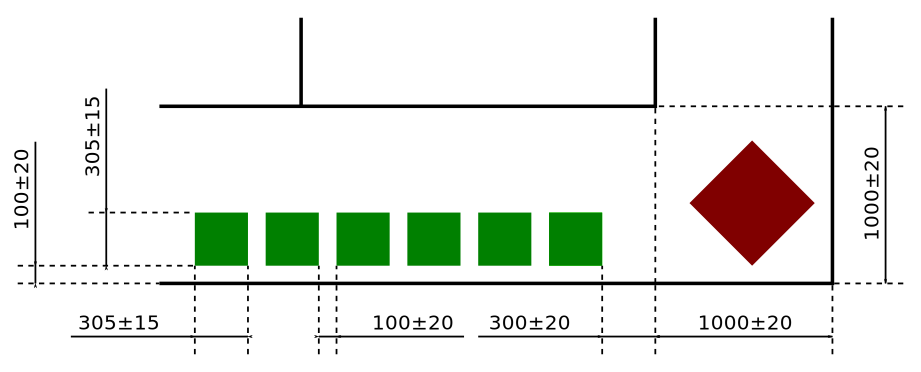
\includegraphics[width=\textwidth]{./images/token-position.pdf}
  \caption{Two perpendicular rows of four $200 \pm 15mm$ wide tokens are spaced evenly $300 \pm 20mm$ to the left and right of the robot's starting boundaries, along the arena walls.
    The tokens are placed $200 \pm 20mm$ away from each other, and $100 \pm 20mm$ from the arena wall.
           All dimensions are in millimetres.}
  \label{fig:token-position}
\end{figure}

\end{enumerate}

\clearpage

\newpage
\section {Awards}
\label{sec:Awards}

\subsection{Main Competition Awards}
Prizes will be awarded to the teams that are placed highest at the end of the competition.  The teams in $1^{st}$, $2^{nd}$ and $3^{rd}$ place will receive awards.

\subsection{Chairman's Award}
The Chairman's Award is given to the team that displays the most extraordinary ingenuity in the design of their robot. It is not awarded for complexity of design, rather the implementation of a simple and elegant solution to a problem.

\subsection{First Robot Movement}
The team that demonstrates the first moving robot to the community will be awarded with an edible prize at the final competition.
\begin{enumerate}
\item The robot movement must be controlled by software running on the Student Robotics kit.
\item The robot must move 1 metre and come to a halt without interference.
\item Proof will be obtained by uploading a video of the robot onto a public sharing site (e.g. youtube.com, flickr.com)
\end{enumerate}


\subsection{Online Presence}
The team that is judged to have the best online presence will be awarded with an edible prize at the final competition.  An online presence is a publicly available set of web pages detailing the team's progress, it can involve blog posts, pictures and videos of the team and the robot.  \emph{Hint: Useful sites include blogger.com, wordpress.com, flickr.com and youtube.com}
\begin{enumerate}
\item When detailing activities online do not post any private information concerning yourself or others.
\item Notify your mentor or email the location of your online materials to \linebreak\href{mailto:info@studentrobotics.org}{\nolinkurl{info@studentrobotics.org}}
\end{enumerate}


\renewcommand{\labelenumi}{\rcn}

\section{Clarifications}
Requests for rule clarifications may be sent to \href{mailto:info@studentrobotics.org}{\nolinkurl{info@studentrobotics.org}}.
Requests received within one month of the competition are unlikely to be processed.

%% The following changes have been made to the rules since their initial release:

\begin{enumerate}
\item 2012-11-12: Added the Rookie Award \& made the First Robot Movement Award only available to Rookie teams.
\item 2013-01-08: Clarified the height of a pedestal with regards to the rim around the top.
\item 2013-02-05: Clarified that only the robot must fit within a $500mm$ cube before the start of a match. A token placed in/on the robot is not included.
\end{enumerate}

\newpage
\appendix
\appendixpage
\addappheadtotoc
\section {Return of Kit}
\label{sec:kit-return}

Each kit issued by Student Robotics contains a manifest which lists the parts and part numbers issued to each team.
Each team is responsible for ensuring that they return the items listed on their manifest.

\subsection {Items to be Returned}

\begin{itemize}
 \item Really Useful Box
 \item Compartment Box
\end{itemize}

\begin{itemize}
 \item Power Board
 \item Motor Board $\times 2$
 \item Servo Board
 \item JointIO Board
 \item $  1m$ CAT5 (SRIC) cable $\times 2$
 \item $0.5m$ CAT5 (SRIC) cable $\times 4$
 \item $0.3m$ CAT5 (SRIC) cable $\times 3$
\end{itemize}

\begin{itemize}
 \item USB Hub
 \item USB Memory Stick
 \item Webcam
 \item USB A to USB Mini B lead
\end{itemize}

\begin{itemize}
 \item Lithium Polymer Battery $\times 2$
 \item Battery Cable (used for connecting a battery to the power board)
 \item IMAX B6 Battery Charger
 \item Charger Power Supply and Mains Cable
 \item Battery charging bag
\end{itemize}

\subsection {When and How to Return Kit}

The kit should be returned at the competition.
If you wish to keep the kit beyond the competition, then this \textbf{must} be arranged with us,
 before the 14\textsuperscript{th} of March 2013, via email to \href{mailto:info@studentrobotics.org}{\nolinkurl{info@studentrobotics.org}}.


\end {document}
